\chapter{Random Processes, Spectra and Sensor Noise}
\label{ch:processes}
\chaptermark{Random Processes and Noise} % short running header

\begin{objectives}
\begin{itemize}
  \item Describe noise that evolves in time: random sequences, autocorrelation, stationarity, white noise and random walks.
  \item Understand power spectral densities and why sensor noise is specified in units per $\sqrt{\mathrm{Hz}}$.
  \item Understand continuous-time white noise, its sampling, and aliasing.
  \item Derive how integrated noise grows, and how covariance evolves in a linear stochastic system.
  \item Derive the Allan variance signatures used to identify IMU noise parameters.
  \item Model colored noise with shaping filters, the reason sensor biases become filter states.
\end{itemize}
\end{objectives}

\Cref{ch:prob} dealt with random vectors: a fixed number of uncertain quantities. Sensor noise is a different kind of object: a random
\emph{signal}, a function of time, whose values at different times may or may not be related. This chapter develops the theory of such
random processes, as far as it is needed to understand IMU datasheets, to model sensor errors in a filter, and to discretize those models
correctly.

% ==============================================================================
\section{Random sequences}

\subsection{Definitions}

A \term{random sequence} (discrete-time random process) is a sequence of random variables $x_0, x_1, x_2, \dots$, for example the noise
added to successive IMU samples. One run of the experiment produces one \emph{sample path}; repeating the experiment produces another.
Statistics are taken across this \emph{ensemble} of paths. The \emph{mean function} is $\mu_k = \E[x_k]$ and the \emph{autocovariance}
\begin{equation}
  C(k, j) = \E\big[(x_k - \mu_k)(x_j - \mu_j)\big]
\end{equation}
says how strongly the values at two times are related. A sequence is \term{wide-sense stationary} if its mean is constant and its
autocovariance depends only on the lag, $C(k, j) = C(k - j)$: its statistical character does not change with time.

\subsection{Three fundamental sequences}

\begin{figure}[t]
  \centering
  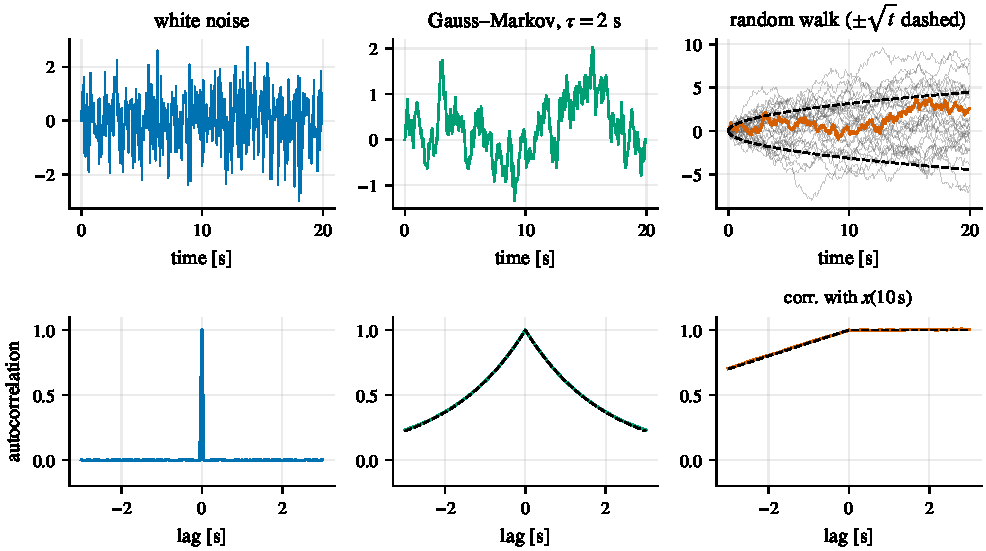
\includegraphics[width=\textwidth]{fig_processes.pdf}
  \caption{Sample paths (top) and autocorrelation functions (bottom) of white noise, a first-order Gauss--Markov sequence with correlation time
  $\tau = 2$~s, and a random walk, all driven by the same white sequence. White noise is uncorrelated with itself at any non-zero lag;
  the Gauss--Markov sequence forgets its past exponentially; the random walk never forgets and its spread grows like $\sqrt t$.}
  \label{fig:processes}
\end{figure}

\paragraph{White noise.} A \term{white sequence} has zero mean and uncorrelated values: $C(k) = \sigma^2$ for $k = 0$ and $0$ otherwise. Each
sample carries no information about the others. The measurement noise of a well-behaved sensor is approximately white.

\paragraph{Random walk.} Summing white noise gives a \term{random walk}: $x_{k+1} = x_k + w_k$, $x_0 = 0$, with $w_k$ white of variance $\sigma^2$. Then
$x_k = \sum_{j<k}w_j$ and, because variances of uncorrelated terms add,
\begin{equation}
  \Var(x_k) = k\sigma^2 .
\end{equation}
The spread grows like $\sqrt k$ without bound, and the sequence is not stationary. Its autocovariance $C(k, j) = \min(k, j)\sigma^2$ shows that
it remembers its whole past. Slowly drifting sensor biases are modeled as random walks.

\paragraph{First-order Gauss--Markov sequence.} Between the two lies $x_{k+1} = ax_k + w_k$ with $|a| < 1$. If the sequence is stationary, taking the
variance of both sides gives $V = a^2V + \sigma^2$, so
\begin{equation}
  \Var(x_k) = \frac{\sigma^2}{1 - a^2}, \qquad C(j) = \frac{\sigma^2}{1 - a^2}\,a^{|j|},
\end{equation}
the second because $x_{k+j} = a^jx_k + (\text{noise uncorrelated with } x_k)$. The sequence forgets its past exponentially, with a
\emph{correlation time} of about $1/(1 - a)$ steps. It is a bounded, slowly varying error: a useful model for biases that wander but do not
diverge, and for many environmental disturbances.

% ==============================================================================
\section{Frequency-domain description}

\subsection{Fourier analysis in brief}

Every reasonable signal is a superposition of sinusoids. The \term{Fourier transform}
\begin{equation}
  X(f) = \int_{-\infty}^{\infty}x(t)\,e^{-i2\pi ft}\,\dd t, \qquad x(t) = \int_{-\infty}^{\infty}X(f)\,e^{i2\pi ft}\,\dd f
\end{equation}
gives the complex amplitude $X(f)$ of the component at frequency $f$ (in Hz). Two facts are all we need. First, Parseval's theorem
$\int|x(t)|^2\dd t = \int|X(f)|^2\dd f$: energy can be counted in time or in frequency. Second, linear time-invariant systems (filters) act
on each frequency independently, multiplying $X(f)$ by a \emph{frequency response} $H(f)$. A low-pass filter has $|H(f)| \approx 1$ at low
frequencies and $|H(f)| \approx 0$ at high ones.

\subsection{Power spectral density}

A random signal has infinite energy (it goes on forever), but finite \emph{power}. Its \term{power spectral density} (PSD) describes how that
power is distributed over frequency.

\begin{definition}[Power spectral density]
For a wide-sense stationary process with autocovariance $C(\tau) = \E[x(t + \tau)x(t)]$ (zero mean), the (two-sided) PSD is
\begin{equation}
  S(f) = \int_{-\infty}^{\infty}C(\tau)\,e^{-i2\pi f\tau}\,\dd\tau .
\end{equation}
\end{definition}

This relation between the autocovariance and the PSD is the \emph{Wiener--Khinchin theorem}. Evaluating the inverse transform at $\tau = 0$ shows
that the variance is the total area under the PSD:
\begin{equation}
  \Var(x) = C(0) = \int_{-\infty}^\infty S(f)\,\dd f .
\end{equation}
So $S(f)\,\dd f$ is the contribution of the frequency band $[f, f + \dd f]$ to the variance, and the PSD has units of $[x]^2/\mathrm{Hz}$. Passing
the process through a filter with frequency response $H(f)$ multiplies its PSD by $|H(f)|^2$.

\begin{pitfall}[one-sided and two-sided PSDs]
Engineers often use a \emph{one-sided} PSD defined only for $f \ge 0$ and equal to twice the two-sided one, so that the variance is
$\int_0^\infty S_1(f)\,\dd f$. Datasheets rarely say which convention they use, and the two differ by a factor of $\sqrt2$ in the noise density.
These notes use the convention of the EuRoC calibration files and of most of the VIO literature: a continuous white noise $w$ with
$\E[w(t)w(s)] = \sigma^2\delta(t - s)$, i.e.\ two-sided PSD $\sigma^2$.
\end{pitfall}

% ==============================================================================
\section{Continuous-time white noise}
\label{sec:ct-noise}

\begin{definition}[Continuous-time white noise]
\index{white noise}
A zero-mean process $w(t) \in \R^n$ is white with \term{noise density} (intensity) $Q_c$ if
$\E[w(t)\,w(s)\T] = Q_c\,\delta(t - s)$, where $\delta$ is the Dirac delta. For a scalar process we write $Q_c = \sigma^2$ and call $\sigma$ the noise
density.
\end{definition}

Continuous white noise is an idealization: its PSD is flat at all frequencies, so its variance $\int S\,\dd f$ is infinite. Physical noise is
white only up to some bandwidth. What makes the idealization useful is that its \emph{integrals} are perfectly well behaved: the integral of
white noise over an interval of length $T$ is a zero-mean random variable with variance
\begin{equation}
  \Var\Big(\int_0^Tw(t)\,\dd t\Big) = \int_0^T\!\!\int_0^T\sigma^2\delta(t - s)\,\dd s\,\dd t = \sigma^2T .
\end{equation}
Since $\delta$ has units of 1/time, $\sigma$ has units of $[w]\cdot\sqrt{\mathrm s} = [w]/\sqrt{\mathrm{Hz}}$. For a gyroscope, $[w] = \mathrm{rad/s}$, so its
noise density is in $\mathrm{rad/s/\sqrt{Hz}}$, the units of \code{gyroscope\_noise\_density} in EuRoC's \code{sensor.yaml}.

\paragraph{From continuous to discrete noise.} A digital sensor reports samples every $\Dt$. If each sample is the average of the
continuous white input over its interval, which an anti-aliasing filter approximates, the sample noise has variance
\begin{equation}
  \Var\Big(\frac1\Dt\int_0^\Dt w(s)\,\dd s\Big) = \frac{\sigma^2}{\Dt}, \qquad \sigma_{\mathrm{discrete}} = \frac{\sigma}{\sqrt{\Dt}} .
  \label{eq:discrete-noise}
\end{equation}
The frequency-domain view agrees: an ideal low-pass filter that keeps the band $|f| < f_s/2$ (with $f_s = 1/\Dt$) passes a variance of
$\int_{-f_s/2}^{f_s/2}\sigma^2\,\dd f = \sigma^2f_s = \sigma^2/\Dt$. Sampling faster does not reduce the noise per unit time; it merely spreads it over
more samples, each noisier. For EuRoC's gyroscope, $\sigma_g = 1.6968\times10^{-4}~\mathrm{rad/s/\sqrt{Hz}}$ at 200~Hz gives a per-sample standard
deviation of $2.4\times10^{-3}$~rad/s.

Conversely, a random walk driven by white noise, $\dot b = w$, gains variance $\sigma^2\Dt$ over a step $\Dt$, so its exact discretization is
$b_{k+1} = b_k + \sqrt{\Dt}\,\sigma\,s_k$ with $s_k \sim \N(0, 1)$. The two conversions go in opposite directions, $\sigma/\sqrt\Dt$ for the sample noise
and $\sigma\sqrt\Dt$ for the walk; confusing them is a classic error in noise simulators.

% ==============================================================================
\section{Sampling and aliasing}

\begin{theorem}[Sampling theorem, Nyquist--Shannon]
\index{sampling theorem}
A signal containing no frequencies at or above $f_s/2$ is completely determined by its samples at rate $f_s$. The frequency $f_s/2$ is the
\term{Nyquist frequency}.
\end{theorem}

\begin{figure}[t]
  \centering
  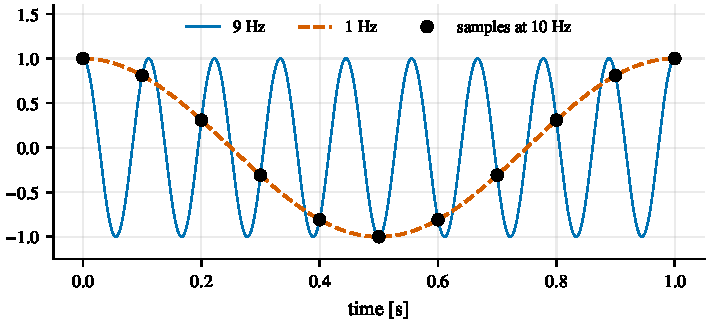
\includegraphics[width=0.9\textwidth]{fig_aliasing.pdf}
  \caption{Aliasing. A 9~Hz sinusoid sampled at 10~Hz (dots) produces exactly the same samples as a 1~Hz sinusoid (dashed). After sampling, the
  two are indistinguishable.}
  \label{fig:aliasing}
\end{figure}

A component at a frequency $f$ above the Nyquist frequency does not disappear when sampled: it masquerades as a lower frequency
$|f - kf_s|$ for the integer $k$ that brings it into $[0, f_s/2]$ (\cref{fig:aliasing}). This \term{aliasing} cannot be undone after sampling, so it
must be prevented before, by an analog or digital \emph{anti-aliasing} low-pass filter. IMUs contain such filters, but strong vibration near
or above the sampling rate (propellers at hundreds of Hz) can still alias into low frequencies and appear as bias-like errors. The same
principle governs images: a camera samples a scene spatially, and an image must be blurred before it is down-sampled, or fine textures turn
into false coarse patterns (\cref{ch:imageproc}).

% ==============================================================================
\section{Integrated noise}

\begin{proposition}[Integrated white noise]
\label{prop:integrated-noise}
Let $w$ be scalar white noise with density $\sigma$. The $m$-fold integral
$I_m(t) = \int_0^t \int_0^{t_1}\cdots\int_0^{t_{m-1}} w(t_m)\,\dd t_m \cdots \dd t_1$ has zero mean and
\begin{equation}
  \Var\big(I_m(t)\big) = \sigma^2\,\frac{t^{2m-1}}{(2m-1)\,\big((m-1)!\big)^2}.
  \label{eq:integrated-noise}
\end{equation}
For $m = 1, 2, 3, 4$ this gives $\sigma^2 t$, $\sigma^2 t^3/3$, $\sigma^2 t^5/20$ and $\sigma^2 t^7/252$.
\end{proposition}
\begin{proof}
By Cauchy's formula for repeated integration (proved by induction, exchanging the order of integration),
$I_m(t) = \int_0^t \frac{(t - s)^{m-1}}{(m-1)!}\,w(s)\,\dd s$. For a weighted integral $\int g(s)w(s)\,\dd s$ of white noise,
$\Var = \iint g(s)g(s')\,\sigma^2\delta(s - s')\,\dd s\,\dd s' = \sigma^2\int g(s)^2\,\dd s$. Here
$\int_0^t (t-s)^{2m-2}\,\dd s/((m-1)!)^2 = t^{2m-1}/((2m-1)((m-1)!)^2)$.
\end{proof}

The single integral $I_1$ is the continuous random walk, or \term{Wiener process}, whose standard deviation grows like $\sqrt t$. Integrating
accelerometer white noise twice into position gives $\sigma_a^2t^3/3$: position uncertainty grows like $t^{3/2}$. Each further integration adds
two powers of $t$ to the variance. \Cref{ch:errordyn} uses this proposition to explain how fast an inertial navigator degrades.

% ==============================================================================
\section{Linear stochastic differential equations}
\label{sec:lyapunov}

Most noise models in navigation are linear systems driven by white noise:
\begin{equation}
  \dot x(t) = F(t)\,x(t) + G(t)\,w(t), \qquad \E[w(t)w(s)\T] = Q_c\,\delta(t - s).
  \label{eq:linear-sde}
\end{equation}
Because white noise is so irregular, such equations are made rigorous by stochastic calculus. For linear systems, however, the results we
need follow from a simple limiting argument.

\begin{proposition}[Mean and covariance propagation]
\label{prop:lyapunov}
\index{Lyapunov equation}
For \eqref{eq:linear-sde}, the mean $m(t) = \E[x(t)]$ and covariance $P(t)$ evolve as
\begin{equation}
  \dot m = Fm, \qquad \dot P = FP + PF\T + GQ_cG\T,
  \label{eq:lyapunov-ode}
\end{equation}
with solution $P(t) = \Phi(t, t_0)P(t_0)\Phi(t, t_0)\T + \int_{t_0}^t\Phi(t, s)G(s)Q_cG(s)\T\Phi(t, s)\T\,\dd s$.
\end{proposition}
\begin{proof}
Over a short interval $h$, $x(t + h) = (I + Fh)x(t) + \int_t^{t+h}Gw\,\dd s + O(h^2)$, and the noise integral is zero-mean with covariance $GQ_cG\T h$ and
uncorrelated with $x(t)$. By \cref{prop:affine}, $P(t + h) = (I + Fh)P(I + Fh)\T + GQ_cG\T h + O(h^2) = P + (FP + PF\T + GQ_cG\T)h + O(h^2)$. Subtract
$P(t)$, divide by $h$ and let $h\to0$. The integral form is verified by differentiating it (\cref{prop:stm}).
\end{proof}

\Cref{eq:lyapunov-ode} is the \emph{Lyapunov differential equation}. The first two terms move and shape the existing uncertainty with the
dynamics; the last term pumps in new uncertainty from the noise. Its integral form over one time step is exactly the discrete process noise
covariance $Q_d$ of the Kalman filter (\cref{ch:linsys,ch:kf}). For a stable time-invariant system, $P$ approaches the solution of the
algebraic Lyapunov equation $0 = FP + PF\T + GQ_cG\T$.

\subsection{The continuous Gauss--Markov process}

The scalar system $\dot x = -x/\tau + w$ with noise density $\sigma$ is the continuous counterpart of the Gauss--Markov sequence. Its stationary
variance solves $0 = -2P/\tau + \sigma^2$:
\begin{equation}
  P_\infty = \frac{\sigma^2\tau}{2}, \qquad C(\Delta t) = P_\infty\,e^{-|\Delta t|/\tau}, \qquad S(f) = \frac{\sigma^2\tau^2}{1 + (2\pi f\tau)^2} .
\end{equation}
(The PSD is the white input PSD $\sigma^2$ times $|H(f)|^2$ for the system's frequency response $H(f) = 1/(i2\pi f + 1/\tau)$; integrating it over all
frequencies returns $P_\infty$.) The autocovariance decays with time constant $\tau$, and the PSD is flat up to the corner frequency $1/(2\pi\tau)$ and
falls off beyond it. Its exact discretization over $\Dt$ is $x_{k+1} = e^{-\Dt/\tau}x_k + w_k$ with $\Var(w_k) = P_\infty(1 - e^{-2\Dt/\tau})$. As
$\tau\to\infty$ it becomes a random walk; as $\tau\to0$ with the low-frequency level $\sigma^2\tau^2$ of its PSD held fixed, it becomes white noise.

% ==============================================================================
\section{Colored noise and state augmentation}

A Kalman filter assumes that its process and measurement noises are white. When a disturbance is \emph{colored} (correlated in time), the
standard remedy is to model it as the output of a linear system driven by white noise, a \emph{shaping filter}, and to add the state of that
system to the filter state. A sensor bias that drifts as a random walk is exactly this: $b$ is colored, but $\dot b = w_b$ is white-driven, so
$b$ becomes part of the state. This is why IMU biases appear in the state vector of every inertial filter (\cref{ch:imu}). Ignoring the
correlation, and treating a slowly varying error as white, makes the filter believe that errors average out when they do not, and leads to
overconfidence.

% ==============================================================================
\section{The Allan variance}
\label{sec:allan}

How are the noise densities of a sensor measured? Record it at rest for hours and compute its \term{Allan variance}, a tool developed for
characterizing atomic clocks that separates noise processes by their time scale.

\begin{definition}[Allan variance]
Split a record of rate samples $y(t)$ into consecutive clusters of duration $\tau$, and let $\bar y_k(\tau)$ be the average over cluster $k$. The
Allan variance is half the mean squared difference of consecutive cluster averages:
\begin{equation}
  \sigma_A^2(\tau) = \tfrac12\,\E\big[(\bar y_{k+1}(\tau) - \bar y_k(\tau))^2\big] .
\end{equation}
\end{definition}

In practice it is computed from the integrated signal $\theta(t) = \int_0^ty$ (for a gyroscope, the angle), since
$\bar y_{k+1} - \bar y_k = (\theta_{k+2} - 2\theta_{k+1} + \theta_k)/\tau$ with $\theta_j = \theta(j\tau)$. The \emph{overlapping} estimator averages over all
starting times rather than only disjoint clusters, which uses the data more efficiently.

\begin{proposition}[Allan variance signatures]
For white noise of density $\sigma$, $\sigma_A^2(\tau) = \sigma^2/\tau$. For a random walk $\dot b = w_b$ with density $\sigma_b$, $\sigma_A^2(\tau) = \sigma_b^2\tau/3$.
\end{proposition}
\begin{proof}
\emph{White noise.} Each cluster average is an integral of white noise divided by $\tau$, with variance $\sigma^2\tau/\tau^2 = \sigma^2/\tau$; consecutive
averages involve disjoint intervals and are uncorrelated, so their difference has variance $2\sigma^2/\tau$, and half of it is $\sigma^2/\tau$.
\emph{Random walk.} Write $b(t) = \int_0^tw_b$. The difference of two consecutive cluster averages is
$D = \frac1\tau\int_\tau^{2\tau}b\,\dd t - \frac1\tau\int_0^\tau b\,\dd t$. Substituting $b$ and exchanging the order of integration expresses $D$ as
$\frac1\tau\int_0^{2\tau}h(s)w_b(s)\,\dd s$ with $h(s) = s$ for $s \le \tau$ and $h(s) = 2\tau - s$ for $s > \tau$ (a triangular weight). Its variance is
$\frac{\sigma_b^2}{\tau^2}\big(\int_0^\tau s^2\dd s + \int_\tau^{2\tau}(2\tau - s)^2\dd s\big) = \frac{2}{3}\sigma_b^2\tau$, and half of it is $\sigma_b^2\tau/3$.
\end{proof}

On a log-log plot of the \emph{Allan deviation} $\sigma_A(\tau)$, independent noise processes therefore appear as straight lines with
characteristic slopes:
\begin{center}\small
\begin{tabular}{@{}l l l@{}}
\toprule
Process & $\sigma_A^2(\tau)$ & slope of $\sigma_A$ \\
\midrule
quantization noise & $3Q^2/\tau^2$ & $-1$ \\
white noise (density $\sigma$) & $\sigma^2/\tau$ & $-\tfrac12$ \\
bias instability ($B$) & $\approx (0.664 B)^2$ & $0$ \\
bias random walk (density $\sigma_b$) & $\sigma_b^2\tau/3$ & $+\tfrac12$ \\
rate ramp ($R$) & $R^2\tau^2/2$ & $+1$ \\
\bottomrule
\end{tabular}
\end{center}
The white-noise density is read off the $-\tfrac12$ line at $\tau = 1$~s, and the random-walk density off the $+\tfrac12$ line at $\tau = 3$~s. The
minimum of the curve marks the averaging time beyond which a stationary sensor's bias starts to wander; its height is related to the
\emph{bias instability}, a flicker-noise floor that neither white noise nor a random walk describes exactly.

\begin{figure}[t]
  \centering
  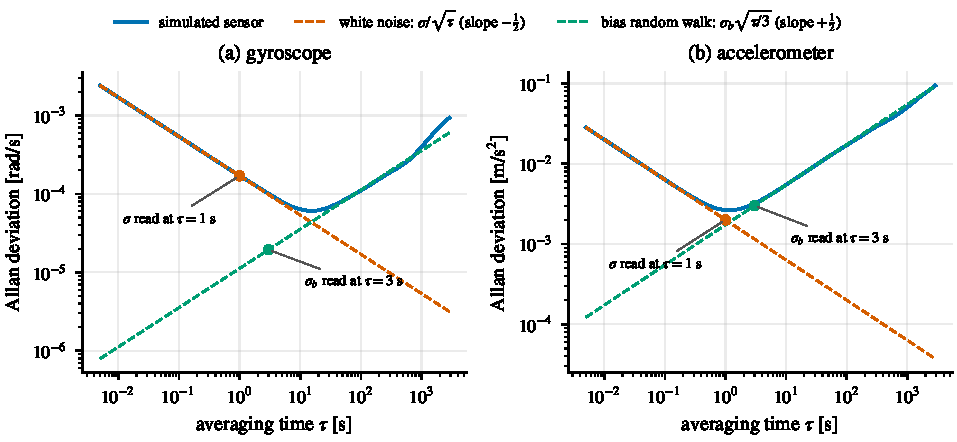
\includegraphics[width=\textwidth]{fig_allan.pdf}
  \caption{Allan deviation of a simulated 4-hour static recording with EuRoC's IMU noise parameters. The $-\tfrac12$ slope of white noise
  dominates short averaging times and the $+\tfrac12$ slope of the bias random walk dominates long ones. Reading the asymptotes at
  $\tau = 1$~s and $\tau = 3$~s recovers the densities.}
  \label{fig:allan}
\end{figure}

\Cref{fig:allan} shows the procedure on simulated data with the EuRoC parameters of \cref{ch:imu}. On real sensors, a flat bias-instability
region appears near the minimum, which the random-walk model only approximates. The IEEE standard procedure~\cite{ieee952} and El-Sheimy et
al.~\cite{elsheimy2008allan} give practical details.

\begin{takeaways}
\begin{itemize}
  \item White noise is uncorrelated in time; a random walk is its running sum, with variance growing linearly; a Gauss--Markov process
        forgets its past exponentially.
  \item The PSD distributes a process's variance over frequency; noise densities are square roots of PSDs, in units per $\sqrt{\mathrm{Hz}}$.
  \item Sampling white noise of density $\sigma$ at period $\Dt$ gives per-sample noise $\sigma/\sqrt\Dt$; a random walk gains $\sigma_b\sqrt\Dt$ per step.
  \item Frequencies above Nyquist alias; filter before you sample or down-sample.
  \item The $m$-fold integral of white noise has variance growing like $t^{2m-1}$.
  \item Covariance in a linear stochastic system obeys $\dot P = FP + PF\T + GQ_cG\T$.
  \item Colored noise is modeled with a shaping filter whose state joins the filter state: this is why biases are states.
  \item The Allan deviation separates white noise (slope $-\tfrac12$, read at 1~s) from bias random walk (slope $+\tfrac12$, read at 3~s).
\end{itemize}
\end{takeaways}

\begin{exercises}
  \item Show that the autocovariance of a random walk is $C(k, j) = \min(k, j)\,\sigma^2$.
  \item For the Gauss--Markov sequence with $a = 0.99$ and $\sigma = 1$, compute the stationary standard deviation and the lag at which the
        correlation drops below $1/e$.
  \item A 1~kHz accelerometer has white noise of $2\times10^{-3}~\mathrm{m/s^2/\sqrt{Hz}}$. What is the standard deviation of a single sample? Of the average
        of 1000 consecutive samples? Of a single sample of the same sensor read at 100~Hz?
  \item A 105~Hz vibration is sampled at 100~Hz. At what frequency does it appear?
  \item Verify \cref{prop:integrated-noise} by Monte Carlo for $m = 2$ and $m = 3$, simulating at 200~Hz for 10~s with 1000 runs.
  \item Solve the Lyapunov equation for the double integrator $\dot p = v$, $\dot v = w$ with $P(0) = 0$ and verify that $P_{pp}(t) = \sigma^2t^3/3$.
  \item Derive the stationary variance and the exact discretization of the continuous Gauss--Markov process.
  \item Simulate 2 hours of a gyro with EuRoC parameters, compute the overlapping Allan deviation, and recover $\sigma_g$ and $\sigma_{b_g}$ from the
        asymptotes. How long a recording is needed to estimate $\sigma_{b_g}$ to 10\%?
\end{exercises}
